\documentclass[a4paper, fontsize=14pt]{article} 
\usepackage{course_work} 
\bibliography{course_work.bib}
%\usepackage{graphs/gnuplot-lua-tikz}
%\setcounter{page}{4} %в зависимости от того, какой по счёту страницей должно быть оглавление!
\usepackage{pstricks}
\begin{document}
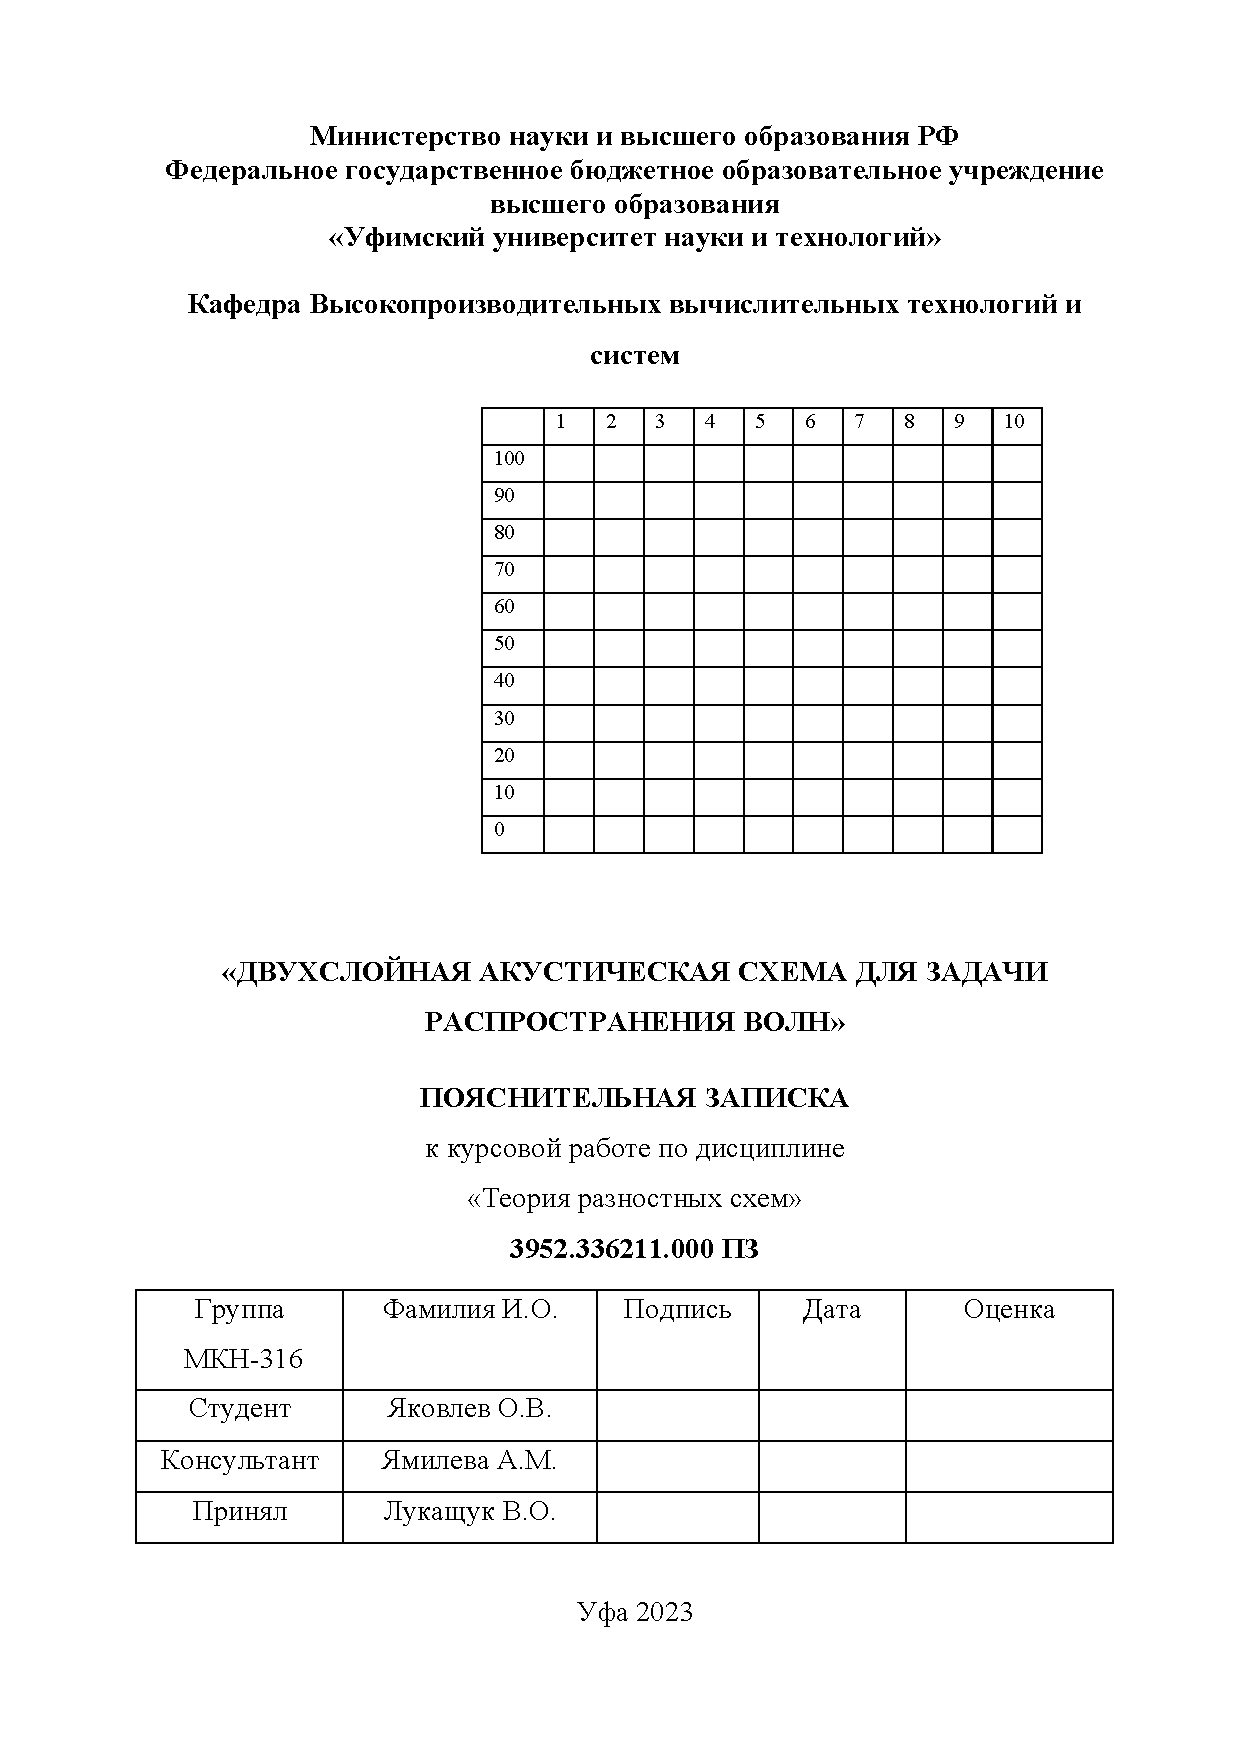
\includepdf[pages=1-3]{cover.pdf}
\newpage
\tableofcontents
\newpage
\section*{Введение}
\addcontentsline{toc}{section}{Введение}
К гиперболическим уравнениям приводят задачи колебания струны, движения сжимаемого газа,
распространения возмущения электромагнитных полей и многие другие. Задачи численного моделирования
распространения акустических волн неоднородной среде часто возникает при геологоразведке различных
месторождений полезных ископаемых. 
% TODO написать еще что-нибудь

Целью данной курсовой работы является изучение распространения акустических волн в неоднородной
среде. Для достижения данной цели были поставлены следующие задачи:
\begin{enumerate}
    \item Изучить литературу по теме "Двухслойная акустическая схема для задачи распространения волн"
    \item Разработать программу для численного решения волнового уравнения в неоднородной среде.
    \item Проанализировать поведение волны на границе сред с разной акустической плотностью.
\end{enumerate}
\newpage
\section{Двухслойная акустическая схема}
\subsection{Одномерная акустическая схема для плоских акустических волн}
Плоские акустические волны описывает уравнение малых колебаний струны при наличии внешнего силового
поля $f$.
\begin{equation}
    \label{strEq}
    \begin{cases}
        \diff[2]{P}{t} = c^2 \diff[2]{P}{x} + f(x,t)\\
        \subs{t=0}{P} = \mu_1(x)\\
        \subs{t=0}{\diff{P}{t}} = \mu_2(x)\\
        \subs{x=0}{P} = \mu_3(t)\\
        \subs{x=a}{P} = \mu_4(t)\\
    \end{cases}
\end{equation}
Заменим уравнение \ref{strEq} второго порядка системой уравнений первого порядка. Введем потенциалы скоростей и
правой части.
\begin{gather*}
    V(x,t) = \int \limits_0^x \diff{P(\xi,t)}{t} \,d\xi\\
    F(x,t) = \int \limits_0^x f(\xi,t) \,d\xi
\end{gather*}
Тогда функции $P(x,t)$,$V(x,t)$ удовлетворяют системе уравнений \ref{acousticSys}. 
\begin{equation}
    \label{acousticSys}
    \begin{cases}
        \diff{P}{t} = \diff{V}{x}\\
        \diff{V}{t} = c^2 \diff{P}{x} + F(x,t)\\
        \subs{t=0}{P} = \mu_1(x)\\
        \subs{t=0}{V} = \int \limits_0^x \mu_2(\xi) \,d\xi\\
        \subs{x=0}{P} = \mu_3(t)\\
        \subs{x=a}{P} = \mu_4(t)\\
    \end{cases}
\end{equation}

Рассмотрим значения скоростей и давления в узлах равномерной пространственной и временной сеток
сеточных функций 
\begin{gather*}
    \omega_h =\{ih, i=\overline{0..N}\} \\ 
    \omega_\tau =\{i\tau,i=\overline{0..M},\tau = \frac{T}{M}\}\\
    y_i = P(x_i,t), x_i \in \omega_h\\
    \hat{y}_i = P(x_i,t+\tau), x_i \in \omega_h\\
    z_i = V\left(x_i+\frac{h}{2},t\right), i \leq N-1,x_i\in \omega_h\\
    \hat{z}_i = V\left(x_i+\frac{h}{2},t+\tau\right), i \leq N-1,x_i\in \omega_h\\
\end{gather*}

Составим явную акустическую схему, используя шаблон, изображенный на рисунке \ref{acousticTpl}.
\begin{figure}[h]
    \centering
    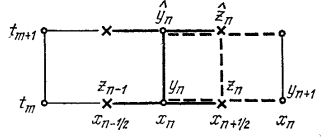
\includegraphics{scheme1d}
    \caption{шаблон одномерной акустической схемы}
    \label{acousticTpl}
\end{figure}
\begin{equation}
    \label{acousticScheme}
    \begin{gathered}
        \frac{\hat{z}_i - z_i}{\tau}=\frac{c^2}{h} (y_{i+1} - y_{i}) + F^{m+1/2}_{i+1/2}, 0\leq i\leq N-1\\
        \frac{\hat{y}_i - y_i}{\tau}=\frac{1}{h}(\hat{z}_i - \hat{z}_{i-1}), 1 \leq i \leq N-1
    \end{gathered}
\end{equation}
При выполнении условия Куранта $c\tau<h$ акустическая схема \ref{acousticScheme} сходится со
скоростью $O(h^2+\tau^2)$  \cite{kal}
\subsection{Двухмерная акустическая схема. Метод FDTD.}
Аналогично одномерному случаю, сведем волновое уравнение второго порядка к системе дифференциальных уравнений
первого порядка.
Главные акустические дифференциальные уравнения для двух измерений имеют вид
\begin{equation}
	\left\{
	\begin{aligned}
		\label{acousticGov}
		\diff{P}{t} =& - c^2\left(\diff{V_x}{x}+\diff{V_y}{t}\right)\\
		\diff{V_x}{t} =& - \diff{P}{x}\\
		\diff{V_y}{t} =& - \diff{P}{y}
	\end{aligned}
	\right.
\end{equation}
Для того чтобы вычислить значения в следующий момент времени, сместим сетки компонент $V_x$ и $V_y$
векторов скоростей относительно сетки давлений $P$ на полшага вдоль соответствующей оси по пространству и на полшага
по времени. В результате узлы сетки будут расположены так, как изображено на рисунке \ref{grid2d}.
\begin{figure}[h]
	\centering
	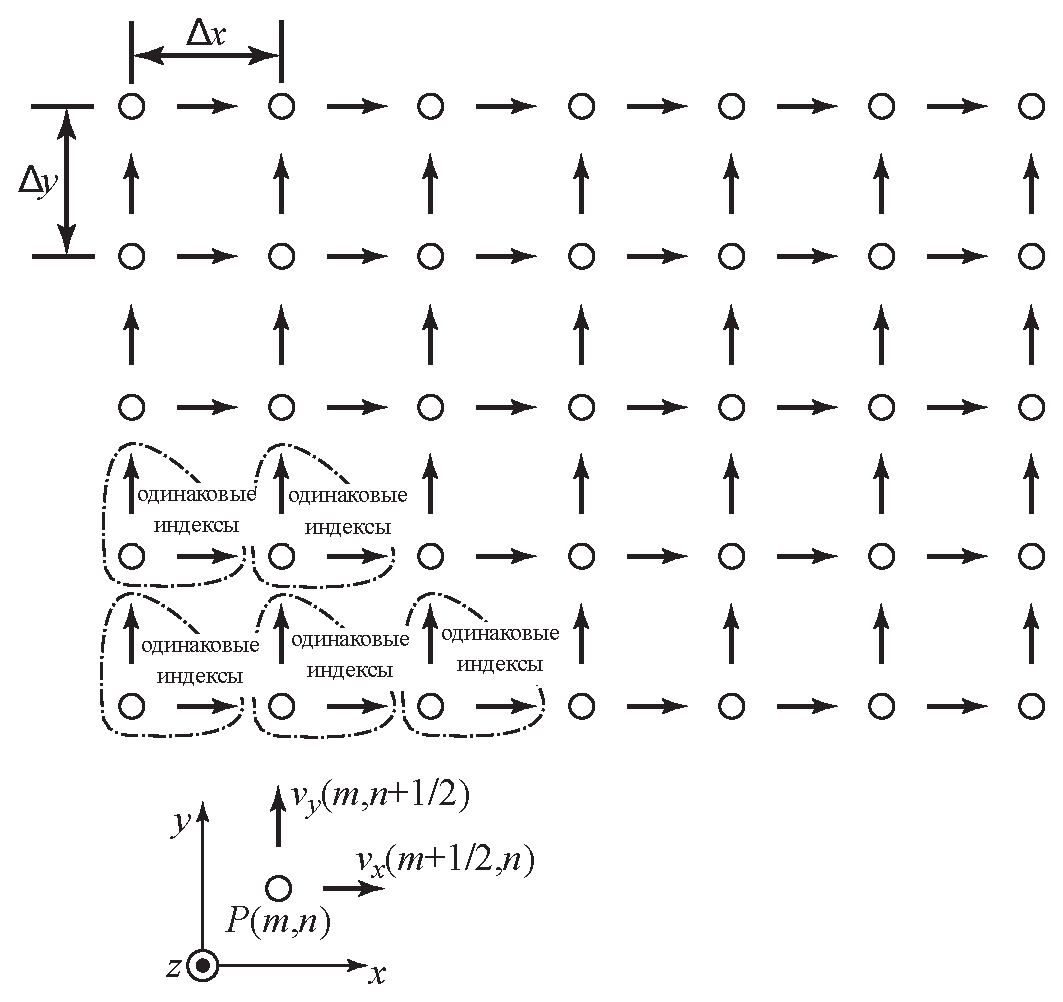
\includegraphics[width=0.75\columnwidth]{acoustic-2d-grid-ru.eps}
	\caption{Расположение узлов в двухмерной сетке}
	\label{grid2d}
\end{figure}

Введем следующие обозначения:
\begin{eqnarray*}
P(x,y,t) & = & P(m\Delta_ta_x,n \Delta_ta_y,  q\Delta_ta_t) \;=\;
 P^q[m,n],\\
V_x(x,y,t) & = & 
  V_x\left([m+1/2]\Delta_x,n \Delta_y,  [q+1/2]\Delta_t\right)
  \;=\; V_x^{q+1/2}[m,n], \\
V_y(x,y,t) & = & 
  V_y\left(m\Delta_x,[n+1/2] \Delta_y,  [q+1/2]\Delta_t\right)
  \;=\; V_y^{q+1/2}[m,n] \\
\end{eqnarray*}
Заменим в системе \ref{acousticGov} производные на разностные аналоги. Тогда давление в следующий
момент времени вычисляется по формуле
\begin{align*}
P^q[m,n] = P^{q-1}[m,n] -
        \rho c_a^2 \frac{\Delta_t}{\delta}
	& \left( V_x^{q-1/2}[m,n]-V_x^{q-1/2}[m-1,n]+\mbox{}\right.\\
	& \left. V_y^{q-1/2}[m,n]-V_y^{q-1/2}[m,n-1]+\mbox{}\right)\\          
V_x^{q+1/2}[m,n] = V_x^{q-1/2}[m,n]
               -\frac{1}{\rho}\frac{\Delta_t}{\delta}
				& \left(P^q[m+1,n]-P^q[m,n]\right)
\end{align*}
Скорость на следующем временном шаге можно вычислить по формулам
\begin{align*}
	V_x^{q+1/2}[m,n] &= V_x^{q-1/2}[m,n]
               -\frac{1}{\rho}\frac{\Delta_t}{\delta}
                \left(P^q[m+1,n]-P^q[m,n]\right)\\
	V_y^{q+1/2}[m,n] &= V_y^{q-1/2}[m,n]
               -\frac{1}{\rho}\frac{\Delta_t}{\delta}
                \left(P^q[m,n+1]-P^q[m,n]\right)\\
\end{align*}

\cite{ufdtd}

\section{Неотражающие граничные условия. PML}
\subsection{Аналитическое продолжение решения}
	Решением волнового уравнения является осциллирующая аналитическая функция. Следовательно, решение
можно аналитически продолжить для всей комплексной плоскости (Рисунок \ref{pmlcont}). Однако, если функцию вычислять не
вдоль действительной оси, а добавить линейно растущую мнимую часть при $\Re x > 5$, то решение будет
экспоненциально затухающее в этой области. То есть, при $\Re x > 5$ функция ведет себя как колебания в
поглощающей среде. 
\begin{figure}[H]
	\centering
	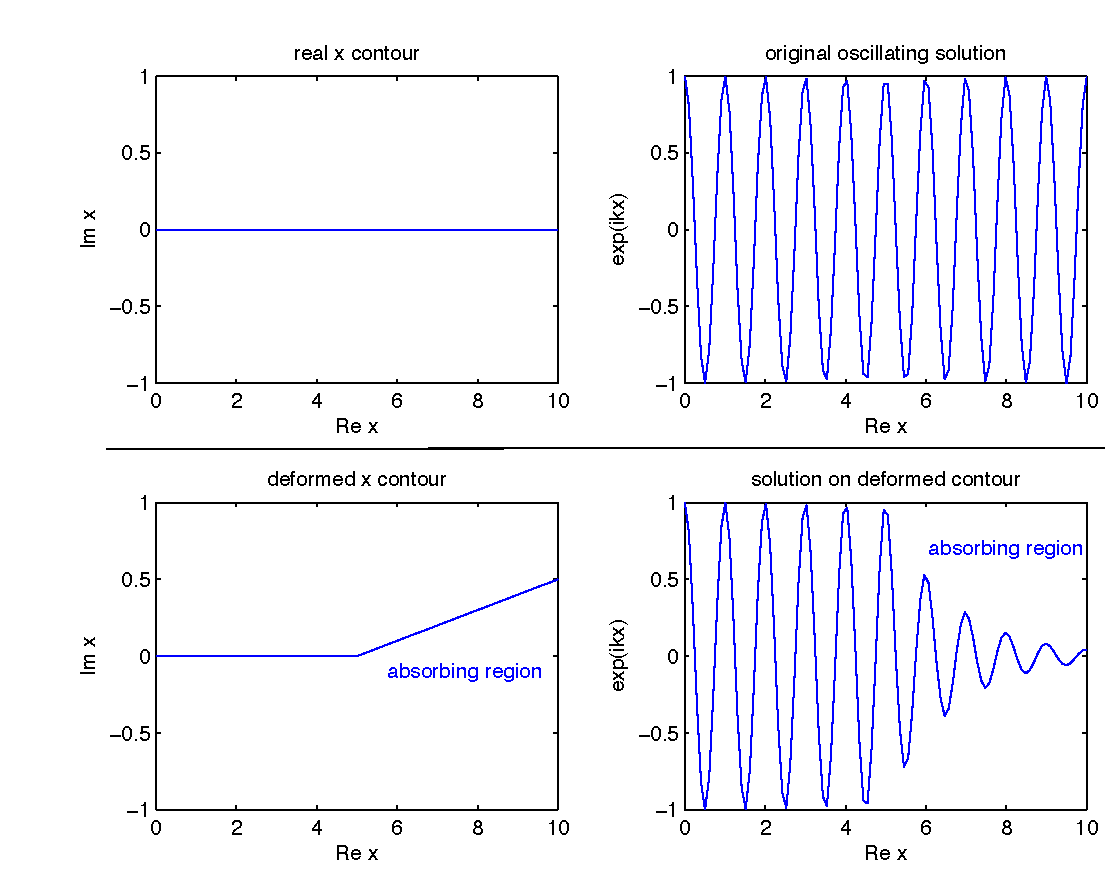
\includegraphics[width=1\columnwidth]{pml-continuation}
	\caption{\emph{Сверху}: действительная часть осциллирующего решения (справа), значения $x$ вдоль
	действительной оси комплексной плоскости $x$ (слева).
	\emph{Снизу}: искривленный контур (слева), экспоненциально затухающее решение (справа). 
	}
	\label{pmlcont}

\end{figure}

При этом решение в области $\Re x < 5$ не изменилось, то есть слой PML ведет себя как неотражающая
поглощающая среда.
\subsection{PML для двухмерных скалярных волн}
Пусть решение $P(x,y,t)$ зависит от времени как $e^{-i \omega t}$. Подставляя в систему
\ref{acousticGov}, получим систему \ref{pmlsys}.

\begin{equation}
	\label{pmlsys}
	\left\{
	\begin{aligned}
		\diff{P}{t} =& -c^2 \left( \diff{V_x}{x} + \diff{V_y}{y} \right) &=& -i\omega P\\
		\diff{V_x}{t} =& - \diff{P}{x} &=& -i\omega V_x\\
		\diff{V_y}{t} =& - \diff{P}{y} &=& -i\omega V_y
	\end{aligned}
	\right.
\end{equation}
Применяя PML-преобразование $\diff{}{x} \mapsto
\frac{1}{1+i\frac{\sigma_x}{\omega}}\cdot\diff{}{x}$, получим 
\begin{equation}
	\label{pmlsystransformed}
	\left\{
	\begin{aligned}
		\diff{P}{t} =& -c^2 \left( \diff{V_x}{x} +
		\diff{V_y}{y}\left(1+i\frac{\sigma_x}{\omega}\right) \right) &=& -i\omega P+\sigma_x P\\
		\diff{V_x}{t} =& - \diff{P}{x} &=& -i\omega V_x+\sigma_x V_x\\
		\diff{V_y}{t} =& - \diff{P}{y} &=& -i\omega V_y
	\end{aligned}
	\right.
\end{equation}
При обратном преобразовании Фурье, выражение $\frac{i}{\omega}\sigma_x \diff{V_y}{y}$ перейдет в
интеграл другой величины. Обозначим его за $\Psi$. Тогда к системе добавляется еще одно уравнение
\begin{equation}
	\diff{\Psi}{t} = -c^2 \sigma_x \diff{V_y}{y}
\end{equation}

	Итоговая система имеет вид
\begin{equation}
	\label{pmlsysfinal}
	\left\{
	\begin{aligned}
		\diff{P}{t} =& -c^2 \left( \diff{V_x}{x} +
		\diff{V_y}{y} \right) -\sigma_x P+\Psi\\
		\diff{V_x}{t} =& - \diff{P}{x} -\sigma_x V_x\\
		\diff{V_y}{t} =& - \diff{P}{y} \\
		\diff{\Psi}{t} =& -c^2 \sigma_x \diff{V_y}{y}
	\end{aligned}
	\right.
\end{equation}
\cite{npml}
\section{Расчет и анализ результатов}
\subsection{Сходимость численного решения}
	Для проверки правильности составленной разностной схемы была выбрана задача \ref{rectmembsys} колебания прямоугольной
мембраны с нулевыми граничными условиями.
\begin{equation}
\label{rectmembsys}
	\left\{
	\begin{aligned}
		&\diff[2]{P}{t}          &=& \diff[2]{P}{x} + \diff[2]{P}{y} \\
		&\subs{x=0}{P}           &=& 0\\
		&\subs{x=1}{P}           &=& 0\\
		&\subs{y=0}{P}           &=& 0\\
		&\subs{y=1}{P}           &=& 0\\
		&\subs{t=0}{P}           &=& \sin \pi x \sin \pi y\\
		&\subs{t=0}{\diff{P}{t}} &=& 0\\
	\end{aligned}
	\right.
\end{equation}
Решением данной задачи является функция $P(x,y,t) = \cos \sqrt{2}\pi t \sin \pi x \sin \pi y$

Вычислим норму ошибки $||E|| = \max\limits_{x_i,y_j \in \omega_h, t_k \in
\omega_\tau} |P^k_{i,j} - P(x_i,y_j,t_k)|$ для численного решения. Норма ошибки в зависимости от
количества узлов пространственной сетки представлен на рисунке \ref{errgraph}.
\begin{figure}[h]
	\centering
	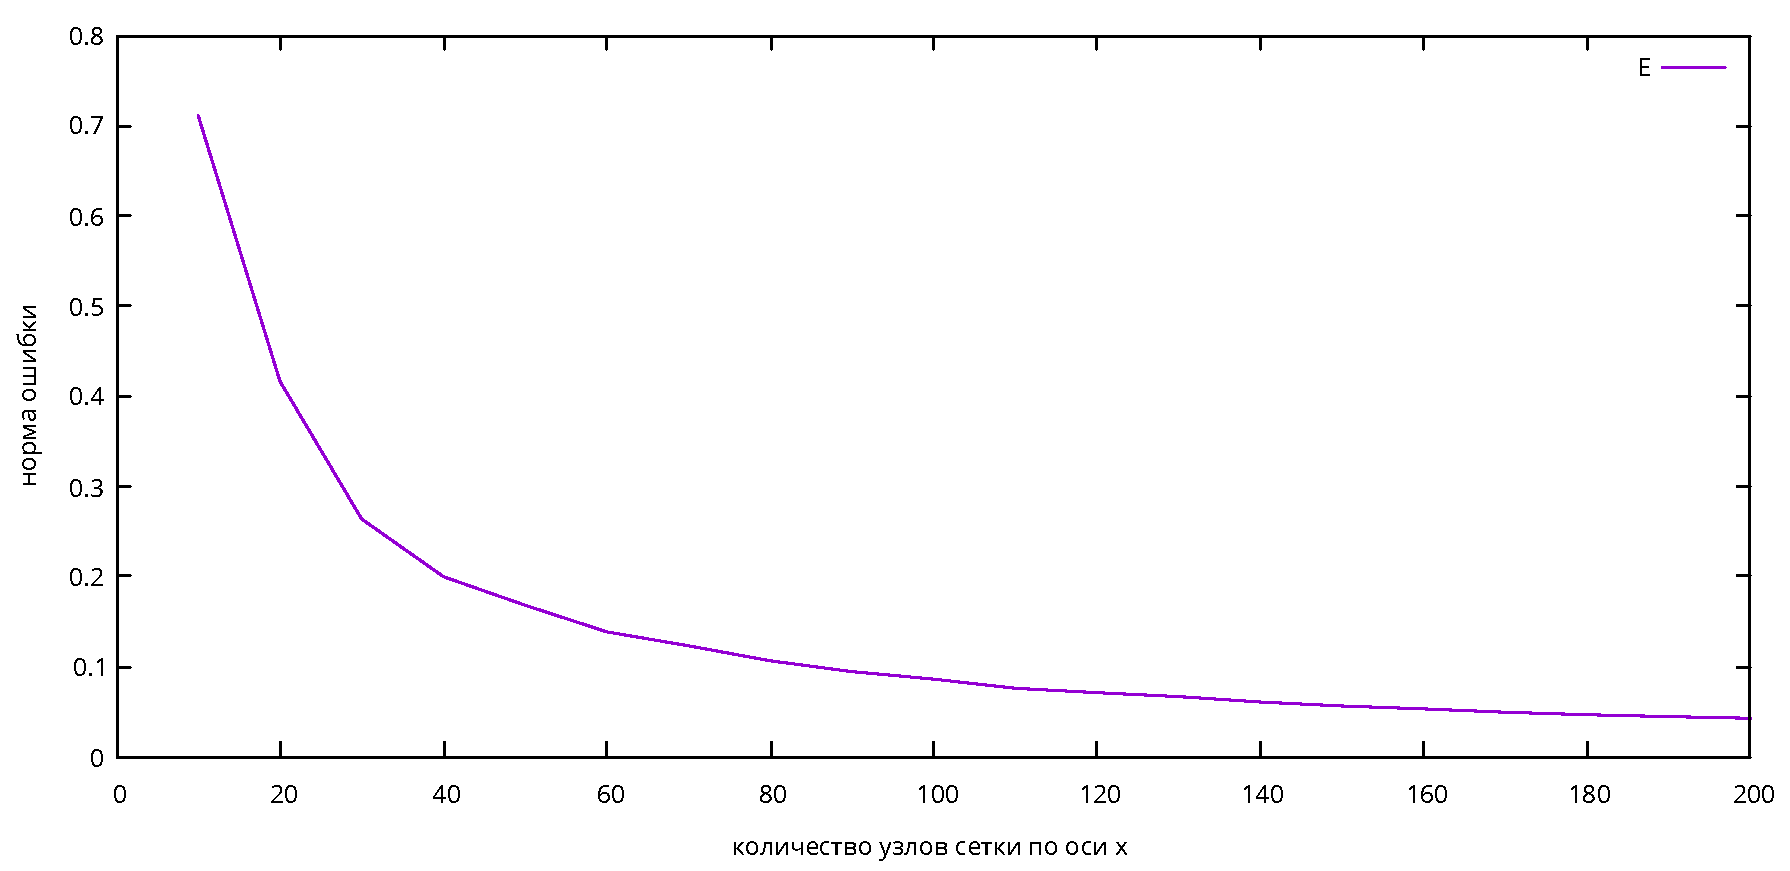
\includegraphics[width=1\columnwidth]{err-graph}
	\caption{Зависимость нормы ошибки от количества узлов сетки по оси $x$}
	\label{errgraph}
\end{figure}
\subsection{Поведение волн на границе сред с разной скоростью звука}
При переходе акустической волны в более акустически плотную среду часть колебаний отражается от
границы раздела сред. На рисунке \ref{wrefl} показано отражение волн, распространяющихся в среде с
со скоростью звука $C_1 = 1$, от границы со средой с меньшей скоростью звука $C_2 = 0.38$.
\begin{figure}[h]
	\centering
	\begin{subfigure}{0.3\textwidth}
		\centering
		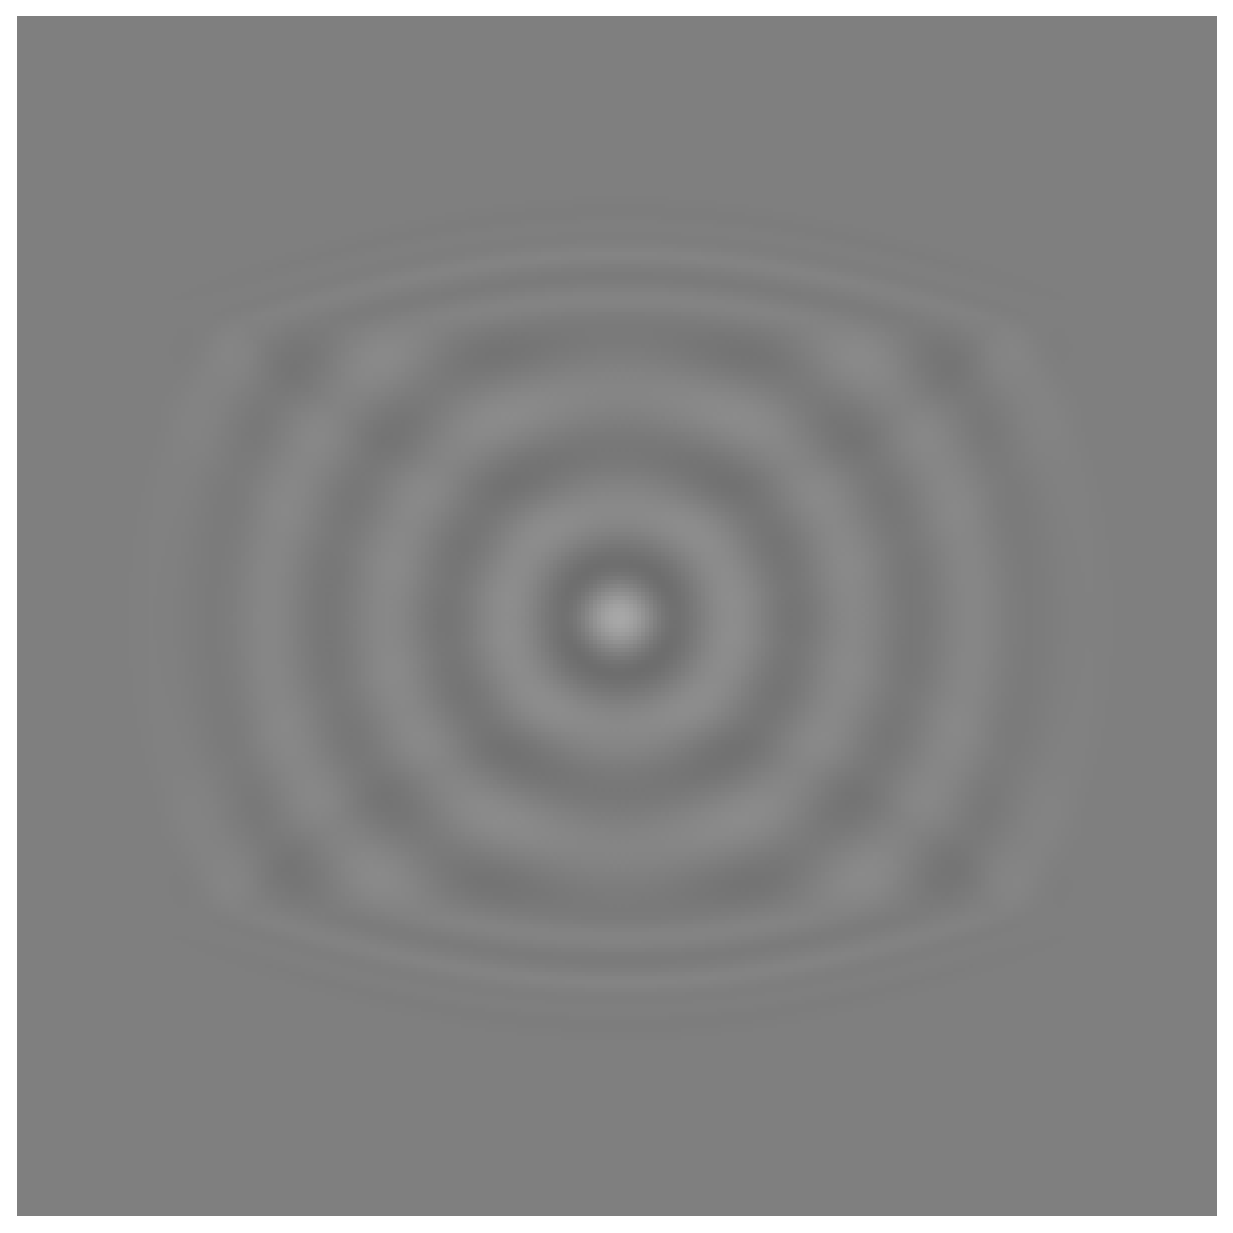
\includegraphics[width=\textwidth]{refl.eps}
		\caption{Отражение}
		\label{wrefl}
	\end{subfigure}
	\begin{subfigure}{0.3\textwidth}
		\centering
		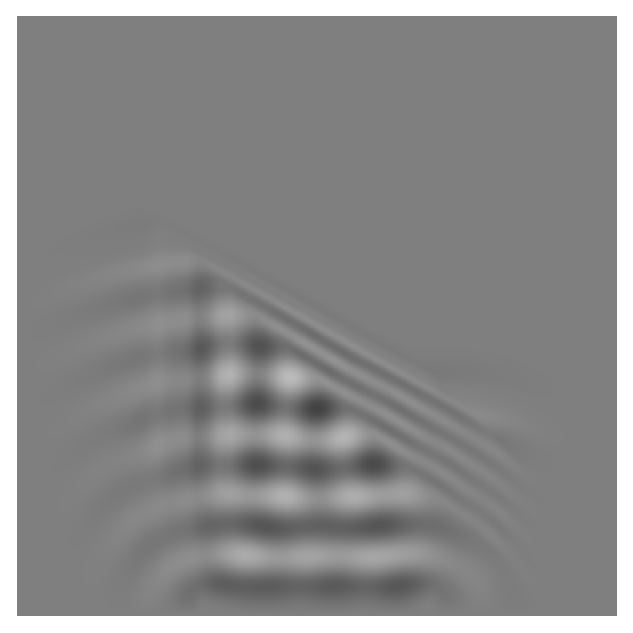
\includegraphics[width=\textwidth]{refr.eps}
		\caption{Преломление}
		\label{wrefr}
	\end{subfigure}
	\begin{subfigure}{0.3\textwidth}
		\centering
		
\includegraphics[width=\textwidth]{difr.eps}
		\caption{Дифракция}
		\label{wdifr}
	\end{subfigure}
    \caption{}
    \label{wphenomena}
\end{figure}

Также, при попадании волны в более акустически плотную среду под углом к границе раздела сред происходит
преломление, изображенное на рисунке \ref{wrefr}. При прохождении волны между границами абсолютно
акустически непроницаемых сред, возникает дифракция волн (рисунок \ref{wdifr}). 

На левой и правой границах вычислительных областей, изображенных на рисунке \ref{wphenomena}, 
расположены неотражающие слои PML c $\sigma_x = e^{8 |x-0.5|}$. Большая часть колебаний при попадании в область PML поглощаются.
Так после отражения от левой границы волны с начальной амплитудой $A_P = 0.1$ амплитуда отраженных
колебаний уменьшается до  $A_P = 0.004$.

\subsection{Задача обнаружения объекта внутри вычислительной области}
В задачах сейсморазведки зачастую необходимо обнаружить область со скоростью звука, отличающейся от
скорости звука в среде. Пусть в центре вычислительной области находится круг радиуса $R$ с со
скоростью звука $C_2 = \frac{1}{4}$ в среде со скоростью звука $C_1 = \frac{1}{2}$. Сенсоры
расположены вокруг объекта. Источник колебаний расположен в середине нижней границы вычислительной области.
Измерим значения давления на датчике, расположенным в точке $\left(\frac{1}{2};\frac{3}{4}\right)$
(отмечен красной точкой на рисунке \ref{detector}).
\begin{figure}[h]
    \centering
    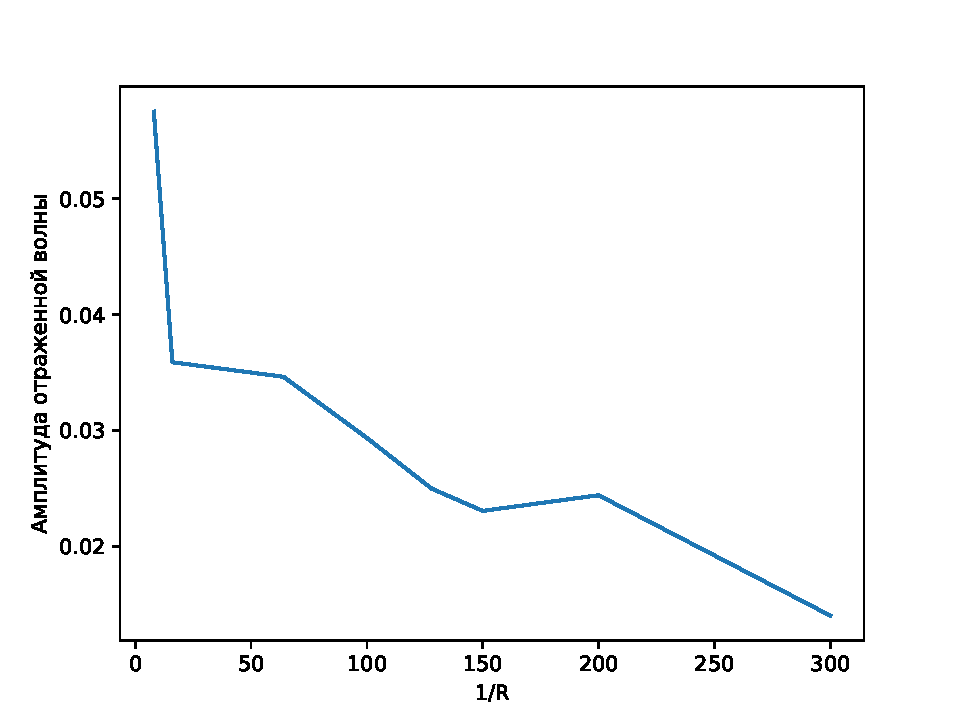
\includegraphics[width=0.6\textwidth]{refl_amp_inv.pdf}
    \caption{}
    \label{reflampinv}
\end{figure}
\begin{figure}
	\begin{subfigure}{0.6\textwidth}
	\centering
    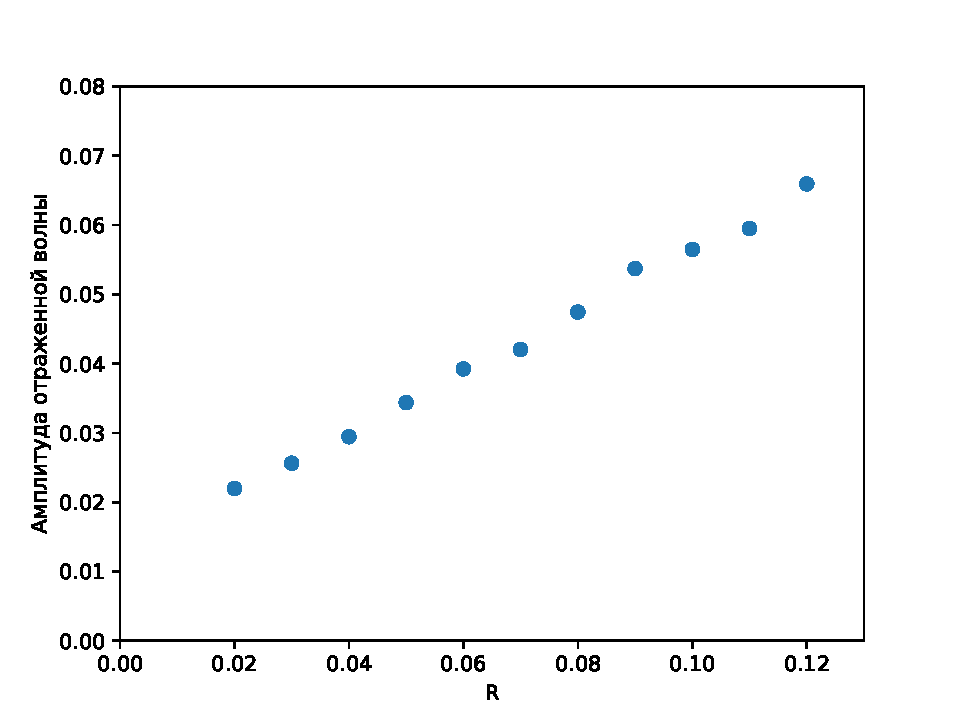
\includegraphics[width=\textwidth]{refl_amp.pdf}
    \caption{Зависимость амплитуды отраженной волны от радиуса круга }
	\label{reflamp}
	\end{subfigure}
	\begin{subfigure}{0.35\textwidth}
	\centering
	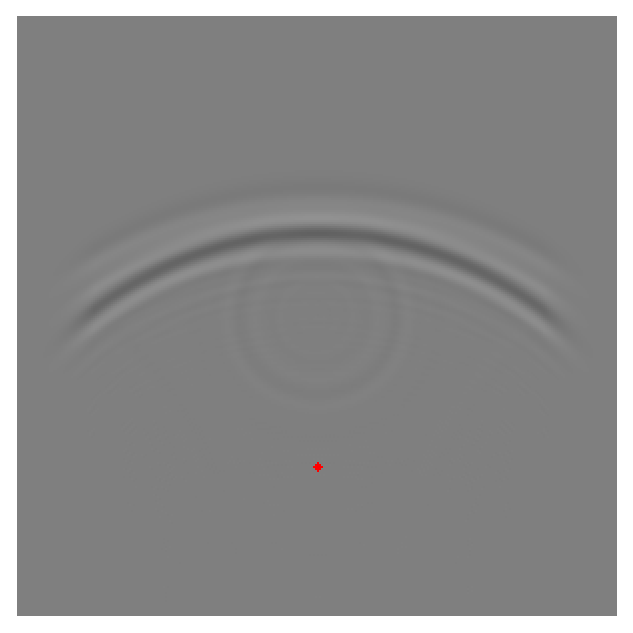
\includegraphics[width=\textwidth]{detector.eps}
	\caption{Отражение от круга радиусом $R=\frac{1}{300}$}
	\label{detector}
	\end{subfigure}

	\begin{subfigure}{\textwidth}
	\centering
	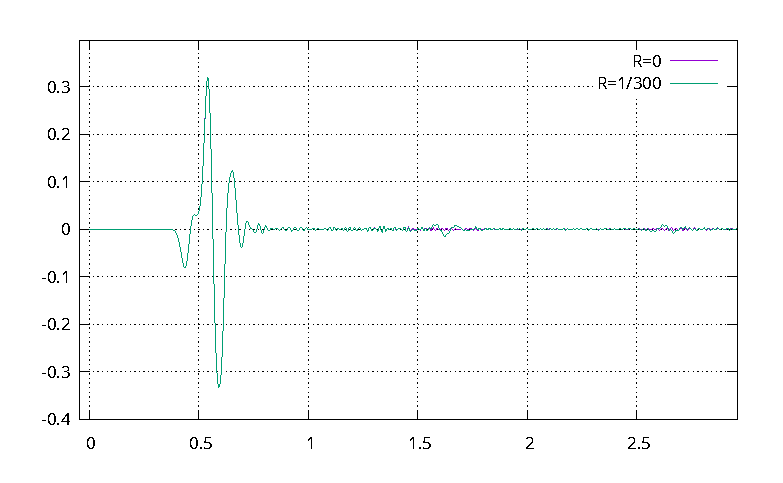
\includegraphics[width=1\textwidth]{sensor.eps}
	\caption{Показания датчика давления, расположенного в точке
	$\left(\frac{1}{2};\frac{3}{4}\right)$, для круга $R = \frac{1}{300}$ и без круга $R=0$}
	\label{sensor}
	\end{subfigure}
    \caption{}
\end{figure}

С уменьшением радиуса круга амплитуда отраженной волны убывает (рисунок \ref{reflampinv}). Так как
волна отражается от границ вычислительной области, что вызывает интерференцию с отраженной волной, 
то существует минимальный радиус круга, который может обнаружить датчик.
Его можно определить при помощи вычислительных экспериментов. Наименьший радиус круга
приблизительно равен $R_\text{min} \approx \frac{1}{300}$ при шаге сетки по пространству $h_x = h_y
= \frac{1}{400}$. Зависимость значения датчика давления от времени представлена на рисунке
\ref{sensor}.

\clearpage

\section*{Заключение}
\addcontentsline{toc}{section}{Заключение}
%
В ходе выполнения курсовой работы была изучена литература по теме <<Двухслойная акустическая схема
для задачи распространения волн>>. Далее была разработана программа для численного решения волнового
уравнения в неоднородной среде. Было проанализировано поведение волны на границе сред с неоднородной
акустической плотностью.

% TODO
Таким образом было изучено распространение акустических волн в неоднородной среде.



\newpage

\addcontentsline{toc}{section}{Список литературы}

\printbibliography

\newpage
\section*{Приложение А}
\addcontentsline{toc}{section}{Приложение А}
\subsection*{Листинг программы}
\lstinputlisting[language=C++]{../problem.hpp}
\lstinputlisting[language=C++]{../waves.cpp}
\lstinputlisting[language=C++]{../problem.cpp}
\lstinputlisting[language=C++]{../problem-detector.cpp}
\lstinputlisting[language=C++]{../problem-difraction.cpp}
\lstinputlisting[language=C++]{../problem-refraction.cpp}
\lstinputlisting[language=C++]{../problem-simple.cpp}
\lstinputlisting[language=C++]{../problem-analytic.cpp}

\includepdf[pages=11]{cover.pdf}

\end{document}
